\begin{frame}{Publicación de un articulo}
\begin{block}{Articulo}
Es comunicar los resultados de investigaciones, ideas, debates, mejoras de manera clara, concisa y fiable.
\end{block}  
\begin{figure}[H]
    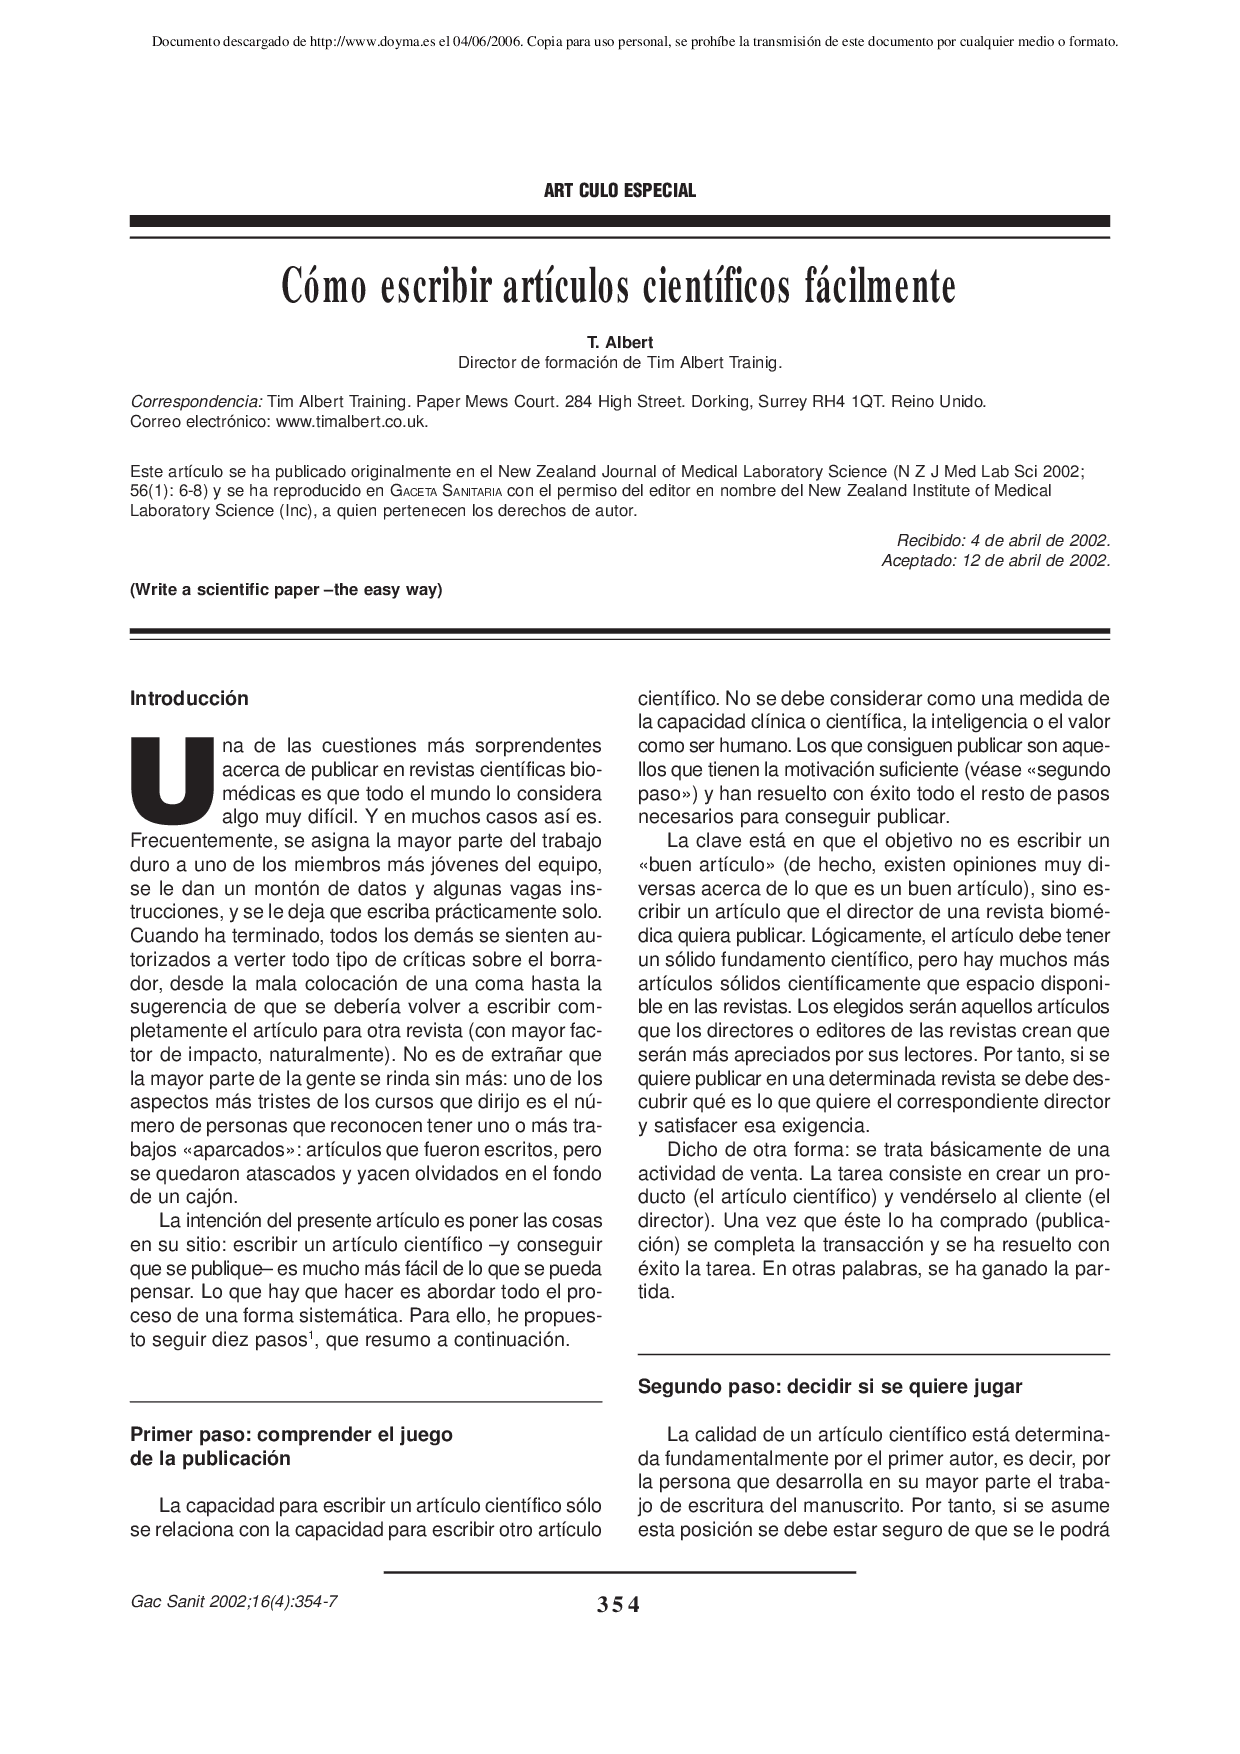
\includegraphics[scale=0.09]{images/articulo.png}
    \label{fig:boat1}
\end{figure}
\end{frame}


\begin{frame}{Revista Indexada}
\begin{block}{}
Publicación periódica de investigación demuestra que una alta calidad ha sido listada en alguna base de datos mundial.
\end{block}   
\begin{figure}[H]
    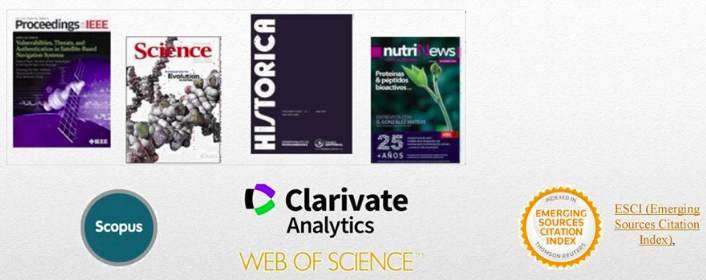
\includegraphics[scale=0.4]{images/revistaindexada.png}
    \label{fig:boat1}
\end{figure}
\end{frame}

\begin{frame}{Proceso}
\begin{block}{}
\begin{enumerate}
    \item Desarrollar un plan (temas de interés)
    \item Elegir una revista
    \item Escribir un articulo
    \item Enviar
    \item Revisar
\end{enumerate}
\end{block}   
\end{frame}

\begin{frame}{Desarrollo del plan}
\begin{block}{Tema de interés}
\begin{itemize}
    \item Elementos originales de tu tesis?
    \item Contribución a la ciencia
    \item Pregunta de investigación
\end{itemize}
\end{block}   
\end{frame}

\begin{frame}{Búsqueda en la Web de Sciense}
\begin{block}{Web de Sciense}
El objetivo es seguir impulsando el uso de la herramienta y dar a conocer las últimas novedades introducidas. [4]
\end{block}   
\begin{figure}[H]
    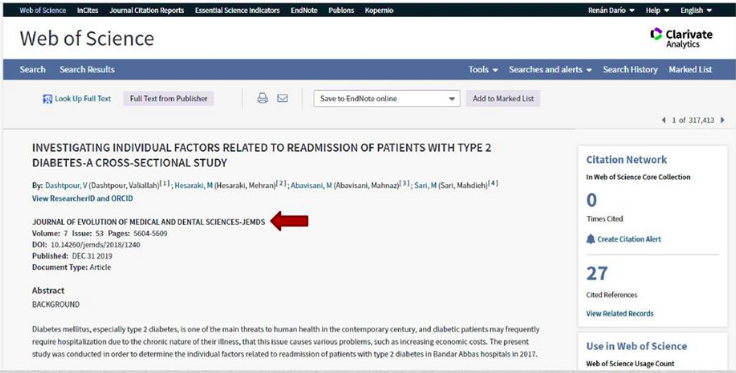
\includegraphics[scale=0.4]{images/webcite.png}
    \label{fig:boat1}
\end{figure}
\end{frame}

\begin{frame}{Búsqueda en scimagojr.com}
\begin{block}{scimagojr.com}
Scimago Institutions Ranking clasifica instituciones directamente vinculadas a la investigación y las posiciona a través de un indicador de síntesis combinando una serie de variables que pertenecen a tres grandes ámbitos: Investigación, Innovación, Impacto social, medido, este último, a través de la visibilidad de sus webs. [6]
\end{block}   
\begin{figure}[H]
    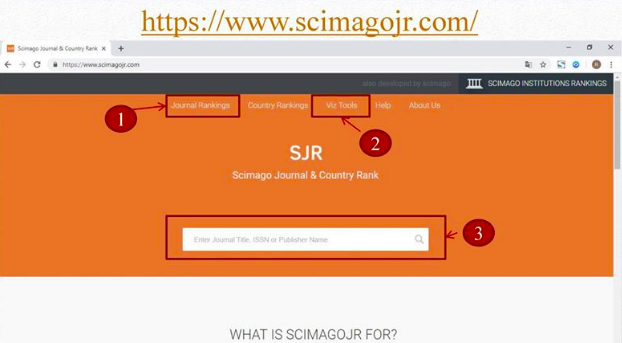
\includegraphics[scale=0.4]{images/webcite2.png}
    \label{fig:boat1}
\end{figure}
\end{frame}

\begin{frame}{Búsqueda en Top Computer Science Conferences}
\begin{block}{Top Computer Science Conferences}
Información de la conferencia, clasificación de la conferencia y métricas (esta es una conferencia TOP). Para hacer la busqueda podemos filtrar por áreas de nuestro interés y por países. [5]
\end{block}   
\begin{figure}[H]
    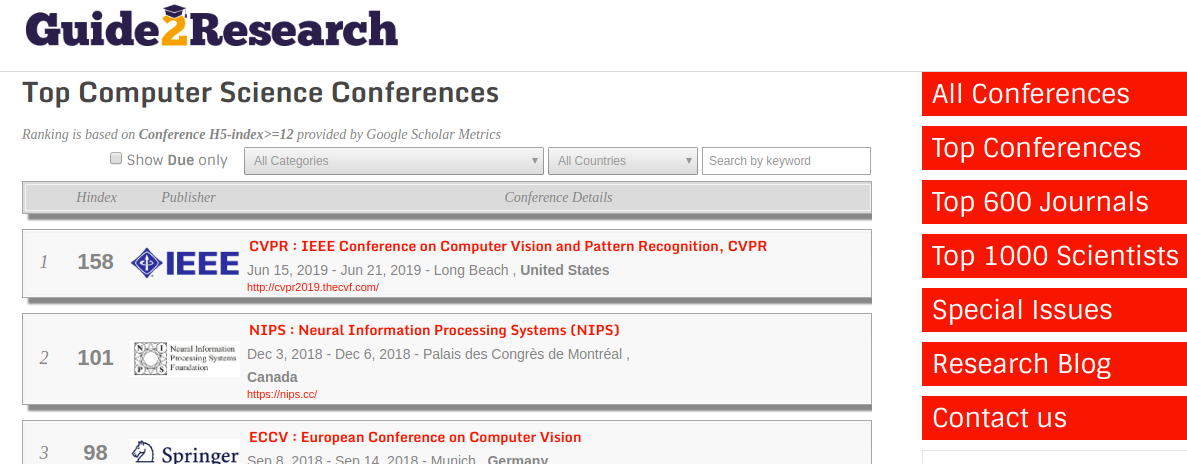
\includegraphics[scale=0.3]{images/top.png}
    \label{fig:boat1}
\end{figure}
\end{frame}

\begin{frame}{Elegir una revista}
\begin{block}{}
\begin{itemize}
    \item Reputación [-]
    \item Reputación [+]
    \item Probabilidad de rechazo [-]
    \item Probabilidad de rechazo [+]
\end{itemize}
\end{block} 
\begin{figure}[H]
    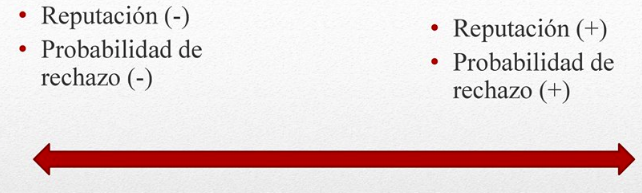
\includegraphics[scale=0.5]{images/paso1.png}
    \label{fig:boat1}
\end{figure}
\end{frame}

\begin{frame}{En la revista escogida debe: }
\begin{figure}[H]
    
\includegraphics[scale=0.5]{images/paso2.png}
    \label{fig:boat1}
\end{figure}
\end{frame}

\begin{frame}{Estructura del articulo}
\begin{block}{}
\begin{itemize}
    \item Titulo 
    \item Autores
    \item Resumen
    \item Introducción
    \item Materiales y métodos
    \item Resultados
    \item Discusión 
    \item Conclusiones
    \item Bibliografía
\end{itemize}
\end{block}   
\end{frame}


\begin{frame}{Consejos}
\begin{block}{}
\begin{itemize}
    \item Ponerse en lugar del lector.
    \item Pedir a un amigo que lo lea.
    \item Presentarlo en una conferencia.
    \item Pide ayuda a una persona con experiencia en publicar.
    \item Si no sabes escribir en otro idioma, utiliza un servidor de traducción.
\end{itemize}
\end{block}   
\end{frame}

